\documentclass{article}
\usepackage{amssymb}
\usepackage{tikz}
\usepackage[margin=4cm]{geometry}

\title{Modelos Discretos: Respuestas tarea 1}
\author{Francisco Carvajal, Vicente Díaz, Benjamín Farías}

\begin{document}
\maketitle



\section{Inducción Estructural}

\section{Inducción sobre strings}

\section{Definición inductiva de grafos}
%Pancho Tarea

\subsection{Mediante inducción estructural defina la estructura del grafo.}
\emph{Lista de naturales:}\\
Definición:
\[ \emptyset \in \mathcal{L}_{\mathbb{N}} \]
\[ L \in \mathcal{L}_\mathbb{N} \Rightarrow L \rightarrow k \in \mathcal{L}_\mathbb{N}, \forall k \in \mathbb{N}\]
Operaciones:
\[ Insertar(L, k) = L \rightarrow k\]


Ejemplos:

\[ \rightarrow 0 \rightarrow 2 \rightarrow 7 \]
\[ Push(\rightarrow 0 \rightarrow 2 \rightarrow 7, 10) =  \rightarrow 0 \rightarrow 2 \rightarrow 7 \rightarrow 10\]
\[ Push(\emptyset, 4) = \rightarrow 4 \]

\emph{Grafo (Direccional):}
\[ \emptyset \in \mathcal{G} \]
\[ G \in \mathcal{G} \Rightarrow G \rightarrowtail (l) \in \mathcal{G} , \forall l \in \mathcal{L}_\mathbb{N} \]

Ejemplos:

\[ \rightarrowtail ( \rightarrow 2 \rightarrow 3) \rightarrowtail (\rightarrow 3) \rightarrowtail (\rightarrow 0) \rightarrowtail (\rightarrow 0 \rightarrow 1) \]
representa el siguiente grafo: 

\begin{center}
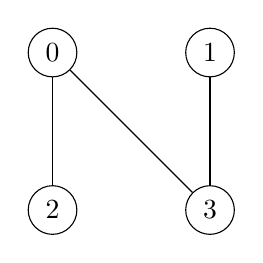
\begin{tikzpicture}
  % Nodos
  \node[circle, draw] (0) at (0,0) {0};
  \node[circle, draw] (1) at (2,0) {1};
  \node[circle, draw] (2) at (0,-2) {2};
  \node[circle, draw] (3) at (2,-2) {3};
  
  % Aristas
  \draw (0) -- (2);
  \draw (0) -- (3);
  \draw (1) -- (3);
\end{tikzpicture}
\end{center}

\subsection{Insertar Nodo}
Esta parte se complica un poco, al ser un grafo no dirigido, ya que, no se puede
solo añadir la lista al final del grafo que ya tenemos, porque se crearia 
asimetria en los datos del grafo, es decir, se puede llegar de j a i, pero 
no de i a j.
Por lo tanto lo que debemos hacer es añadir la lista al final pero ademas 
debemos agregar en cada lista del grafo que corresponda, un borde a la nueva 
arista.
Para hacer esto lo primero que hare es una funcion que conecte el nodo i y j
de un grafo G.

\[ Conectar((L) \rightarrowtail G, 0, j) = (Insertar(L, j)) \rightarrowtail G \]
\[ Conectar((L) \rightarrowtail G, i, j) = (L) \rightarrowtail Conectar(G, i-1, j) \]

Ademas ahora seria util una funcion que conecte una lista de nodos a un nodo,
para utilizarla en la funcion final.

\[ ConectarTodos(G, \emptyset, j) = G  \]
\[ ConectarTodos(G, i \rightarrow L, j) = ConectarTodos(Conectar(G, i, j), L, j)  \]

Ahora que ya podemos conectar el nodo i con el j, necesitamos saber que valor 
tendra j, por lo tanto, tenemos que saber cuantos nodos hay en el grafo para 
conocer cual sera el valor del siguiente.

\[ ContarNodos(\emptyset) = 0 \]
\[ ContarNodos((L) \rightarrowtail G) = 1 + ContarNodos(G) \]

Con estas funciones auxiliares creadas, el trabajo se facilita mucho y ya 
podemos definir la funcion InsertarNodo.

\[ InsertarNodo(G, L) = ConectarTodos(G \rightarrowtail (L), L, ContarNodos(G)) \]

\subsection{Cantidad minima de aristas}

B.I.
\[ a = n - 1 \]

\[n = 1; 1 - 1 = a = 0 :)\]
\[n = 2; 2 - 1 = a = 1 :)\]

H.I.
Asumimos correcto que
\[ a = n - 1 \]

T.I.

\subsection{Cantidad maxima de aristas}

\[ max(a_n) = \frac{n(n-1)}{2} \]

B.I.

\[n = 1; \frac{1(1-1)}{2} = 0 = max(a_0) :)\]
\[n = 2; \frac{2(2-1)}{2} = 1 = max(a_1) :)\]
\[...\]
\[n = 5; \frac{5(5-1)}{2} = 10 = max(a_5) :)\]

H.I.
Asumimos cierto 
\[ max(a_n) = \frac{n(n-1)}{2} \]

T.I.
\[ max(a_{n+1}) = \frac{n(n+1)}{2} = \frac{n^2+n}{2} = \frac{n^2-n + 2n}{2} = \frac{n(n-1)}{2} + n \]
\[ max(a_{n+1}) = max(a_n) + n \]



\section{Inducción para resolver sumatorias}

\section{Inducción sobre fórmulas lógicas}

\section{Inducción sobre números naturales}

\section{Falacias inductivas}

\end{document}
